% this is samplepaper.tex, a sample chapter demostrating the
% LLNCS macro package for Springer Computer Science proceedings;
% Version 2.20 of 2017/10/04
%
\documentclass[runningheads]{llncs}
%
\usepackage{graphicx}
\usepackage{listings}

\usepackage{subcaption}
\usepackage{array}

\usepackage[table]{xcolor}
\usepackage{multirow,bigstrut}
\usepackage{rotating}
%...

%\usepackage{siunitx} % Required for alignment

%\sisetup{
%  round-mode          = places, % Rounds numbers
%  round-precision     = 4, % to 4 places
%}

%..

% Used for displaying a sample figure. If possible, figure files should
% be included %in EPS format.
%
% If you use the hyperref package, please uncomment the following line
% to display URLs in blue roman font according to Springer's eBook style:
% \renewcommand\UrlFont{\color{blue}\rmfamily}

\begin{document}
%
\title{Fuzzy Adaptation of Parameters in a Multi-Swarm Particle Swarm Optimization (PSO) Algorithm Applied to the Optimization of a Fuzzy Controller } 

%
\titlerunning{Fuzzy Adaptation of Parameters in a MS-PSO}
% If the paper title is too long for the running head, you can set
% an abbreviated paper title here
%
\author{Alejandra Mancilla\orcidID{0000-0003-0430-8152} \and
Oscar Castillo\orcidID{0000-0002-7385-5689} \and
Mario García-Valdez\orcidID{0000-0002-2593-1114}}
%
\authorrunning{A. Mancilla et al.}
% First names are abbreviated in the running head.
% If there are more than two authors, 'et al.' is used.
%
\institute{Tijuana Institute of Technology / Tecnologico Nacional de Mexico, Tijuana, Mexico\\
    \email{\{alejandra.mancilla,mario\}@tectijuana.edu.mx,ocastillo@tectijuana.mx}}

%
\maketitle              % typeset the header of the contribution
%
\begin{abstract}

     Many control problems require running many simulations to establish the optimal parameters for the controller. One option is to use population-based distributed algorithms. A common configuration is to employ multiple independent populations to run parallel search algorithms, with each population running in an independent processor. One issue with these algorithms is finding the ideal configuration to improve their performance, such as the number of populations, the number of processors, and particularly the parameters that affect exploration and exploitation in the search. In this work, we suggest a version of multi-swarm Particle Swarm Optimization (PSO) that includes a Fuzzy Inference System (FIS) to dynamically adjust the algorithm's parameters. The adjustment considers two variables: population diversity and the number of iterations performed on the population. As an output of the FIS, we obtain the adapted parameters, representing the new values for the social coefficient and the cognitive coefficient to be used in the next iteration. We aim to evaluate if this strategy helps minimize the evaluation time and minimize the root-mean-square error (RMSE). As a case study, the distributed PSO algorithm is applied to optimize the membership functions of a fuzzy controller for tracking the trajectory of an autonomous mobile robot. The results indicate that the proposed strategy for optimizing the algorithm's parameters achieves an RMSE similar to the results found in previous works.

\keywords{Fuzzy Control \and Distributed Algorithms \and Parameter Adaptation}
\end{abstract}
%
%
\section{Introduction}

In a recent paper, we presented a distributed algorithm for multi-population
metaheuristics \cite{mancilla2022optimal,mancilla2022tracking} using Genetic
Algorithms (GAs) \cite{back1996evolutionary,holland1992adaptation} and Particle
Swarm Optimization (PSO) \cite{kennedy2006swarm,clerc2010particle}. We execute
this algorithm asynchronously using a queue-based architecture
\cite{valdez2021container,merelo2018introducing}. One of the problems of using
a multi-population multi-heuristic approach is that we need to set the
algorithms' parameters for each population \cite{ma2019multi}. Finding these
parameters is time-consuming because we need to run several experiments trying
different configurations until we find a suitable parametrization. This problem
could be especially problematic if we have a multi-population algorithm
consisting of several small populations, each with a set of initial parameters
we need to set.

To tackle this problem, in the past, we followed a homogeneous
approach \cite{Mancilla2021}, simply using the same set of parameters for all
populations. In this case, we have two types of algorithms: some populations
run a GA while others execute a PSO. This situation adds another layer to the
problem because each algorithm requires different parameters. In this work, we
compare two strategies to set the initial parameters of the algorithms of the
multi-populations. The first is a homogeneous approach with fixed values, and
the second is a heterogeneous strategy selecting random values from a
predefined range of values established for some of the parameters of the
algorithms \cite{gong2011distributed,hernandez2017randomized}. 

We organized this paper as follows. First, in Section \ref{sec:experiments}, we
describe our proposal and define the experimental setup consisting on
optimizing a fuzzy rear-wheel controller using different configurations on a
benchmark problem. We show and discuss the results in Section
\ref{sec:results}. Finally, we present our conclusions and future work in
Section \ref{sec:conclusions}.

\section{Methodology and Experimental Setup}\label{sec:experiments}

Multi-swarm optimization is a variant of particle swarm optimization (PSO) based on the use of multiple sub-swarms instead of one (standard) swarm.

This adds new design choices not found in a single swarm:

\begin{itemize}
    \item Each swarm can have a different configuration.
    \item Size of each swarm.
    \item How swarms communicate.
    \item How often.
    \item Non-random initial position of particles.
\end{itemize}

\textbf{Exploitation} considers the information obtained from the best solutions found so far.  
C1 (Cognitive Coefficient) controls how much the best personal  solutions influence the swarm. 
\textbf{Exploration} helps discover unexplored regions and avoid premature convergence. 
C2 (Social Coefficient) controls how much the best global solution influences the swarm.
Achieving a balance between these two parameters is a critical problem facing most current search and optimization techniques. 

In this work, we propose a new fuzzy strategy to improve the balance between exploration and exploitation in the Particle Swarm Optimization algorithm. We analyzed how two versions of a distributed parametrization strategy behave in this kind of problem, so we can use this approach in future research. We aim at refining its design and improving the overall performance.

In this work, we use a technique called Dynamic Parameter Adaptation.It is a technique widely used today to improve the performance of bio-inspired algorithms. The idea is to change the values of the parameters while the algorithm is in execution, to get better results. In this work, a fuzzy inference system is used for adapting the parameters.

It is important that the exploration of the solution space is carried out correctly, for which it is necessary to maintain in the population individuals with different characteristics that represent the majority of the search space.  This means, that we must maintain a diversity in the population (Fig.  \ref{fig:diversity}). Therefore, if we have a low diversity it means that the particle is exploiting the search space, if the diversity is high it means that the search space is being explored. In a search algorithm, a high diversity is desired at the \textbf{beginning} of the run. While a low diversity is desired at the \textbf{end} of the run.

\begin{figure}
  \centering
  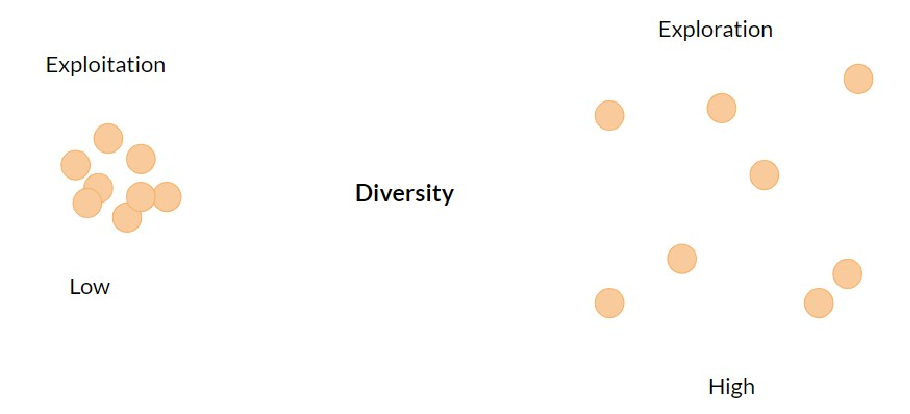
\includegraphics[angle=0,width=1\textwidth]{diversity}
  \caption{Dynamic Parameter Adaptation}
  \label{fig:diversity} 
\end{figure}


As an example, in a single swarm algorithm (Fig. \ref{fig:generation}).
We want to have a high diversity at the beginning of the run.  There is high diversity when we start, because each particle is created with random values, and from there, diversity  begins to decrease as the algorithm advances, in which case the particles begin exploring and ends up exploiting the search space.

If the generation is low, that is, it is starting, the cognitive coefficient (C1) is set to low, and the social coefficient (C2) will be set to high because we want exploring  particles.

\begin{figure}
  \centering
  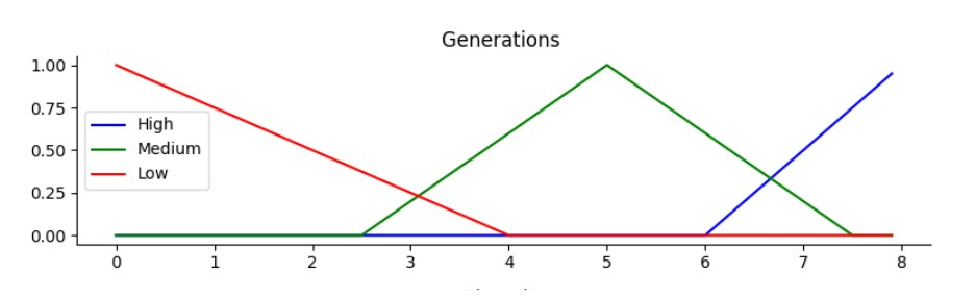
\includegraphics[angle=0,width=1\textwidth]{FM generation.pdf}
  \caption{IF Generation is LOW then C1 is LOW and C2 is HIGH}
  \label{fig:generation} 
\end{figure}

We define a FIS to adapt the coefficients C1 and C2 of the PSO algorithm, in which we have the number of cycles and diversity as input variables, and C1 and C2 as output variables.
On the right side we see an example of how diversity changes in each generation in a PSO algorithm. We measure the diversity and adjust C1 and C2 accordingly, this is done for each cycle defined in the combiner phase, in each swarm.

As we have mentioned, we can do the parameter adaptation in each iteration of the local PSO, but we can also do it in each cycle of the combiner. For our work we experimented  with both strategies and based on the results we decided to do the parameter adjustment by cycles because it gave similar results (Fig. \ref{fig:adap}).

\begin{figure}[ht]
  \centering
  \begin{subfigure}{0.8\textwidth}
    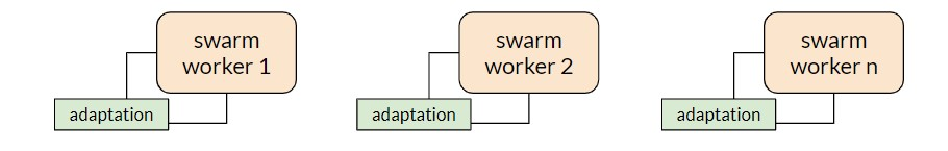
\includegraphics[angle=0,width=1\textwidth]{adaptation local.pdf}
    \caption{Adaptation can be on each iteration on the local PSO.}
    \label{fig:adap_local} 
  \end{subfigure}

  \begin{subfigure}{0.8\textwidth}
     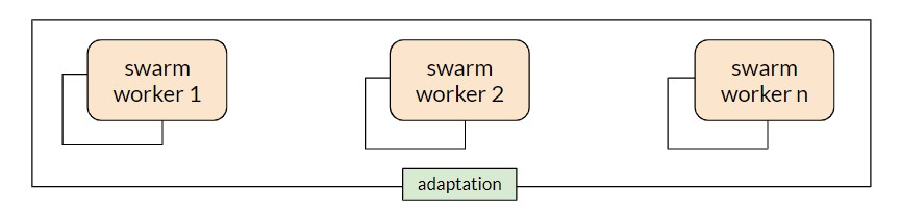
\includegraphics[angle=0,width=1\textwidth]{adaptation combiner.pdf}
     \caption{Adaptation can be done on each cycle of the combiner.}
     \label{fig:adap_combiner} 
  \end{subfigure}
\caption{Strategies for parameter adjustment.}
\label{fig:adap}
\end{figure}

Here we have the multi swarm design, in which multiple swarms are created and added to an Input queue, these swarms are then evolved by multiple workers , and finally they migrate in the combinator process. This cycle is repeated a number or times. The dynamic adaptation of C1 and C2 is executed each time a swarm reaches the combinator.

Here we have the membership functions of the input and output variables (Fig. \ref{fig:member}). 
We tested and found that the diversity for our use case is less than 20. And the number of cycles is 10. C1 and C2 are defined between 1 and 2.

\begin{figure}
  \centering
  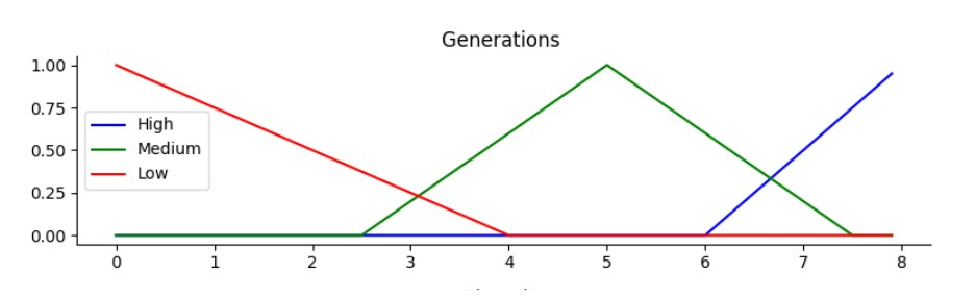
\includegraphics[angle=0,width=1\textwidth]{FM generation.pdf}
  \caption{Membership Functions}
  \label{fig:member} 
\end{figure}

With these variables, we proposed a controller with nine fuzzy rules. We show in the Table \ref{tab:fuzzy_rules}. 

\begin{table}[ht] 
\caption{Fuzzy Rules}\label{tab:fuzzy_rules}
\setlength{\tabcolsep}{10pt}
\begin{tabular}{l l l l l l l}
\hline
\textbf{Algorithm} & \textbf{Parameter}	& \textbf{Range [min,max]}\\ \hline
PSO & Topology & Fully connected  \\
& Speed limit  & Min=[-0.20, -0.30] \\
&              & Max=[0.20, 0.30]  \\
& Cognitive and Social $C_1,C_2$ &  [1.0, 2.0]  \\ \hline
Polutations & Pop Size                & 10  \\
            & Number of Swarm         & 16 \\
            & Number of Generation    &  8 \\
            & Number of Cycles        & 10   \\
            & Number of Parameters    & 15   \\   
            & \#Func. Eval.           & 12800 \\ \hline
\end{tabular}
\end{table}
\subsection{Use Case}\label{sub:use_case}

Here we have the optimization use case. We optimize the membership functions for a benchmark control problem. A rear-wheel controller described by Paden et al.

The parameters of the distributed PSO algorithm are shown in this Table  \ref{tab:alg_params}.
We setup the algorithm with sixteen swarms with ten particles each. Each worker will run eight iterations (generations) of the algorithm before returning the swarm to the output queue. All swarms will complete ten cycles; this means that they will go through the combiner ten times.


\begin{table}[ht] 
\caption{Experimental Setup}\label{tab:alg_params}
\setlength{\tabcolsep}{10pt}
\begin{tabular}{l l l}
\hline
\textbf{Algorithm} & \textbf{Parameter}	& \textbf{Range [min,max]}\\ \hline
PSO & Topology & Fully connected  \\
& Speed limit  & Min=[-0.20, -0.30] \\
&              & Max=[0.20, 0.30]  \\
& Cognitive and Social $C_1,C_2$ &  [1.0, 2.0]  \\ \hline
Polutations & Pop Size                & 10  \\
            & Number of Swarm         & 16 \\
            & Number of Generation    &  8 \\
            & Number of Cycles        & 10   \\
            & Number of Parameters    & 15   \\   
            & \#Func. Eval.           & 12800 \\ \hline
\end{tabular}
\end{table}

\section{Results}\label{sec:results}

In Table \ref{tab:rmse}, we show the results of the experiments. The distributed results with parameters with dynamically adjusted values are compared against a distributed version initialized with random parameters for each swarm; this is found in our previous work.

We can note that the distributed PSO with dynamic parameter adaptation implementation yields better results than the distributed heterogeneous parameters on average. Here we show the average ERROR obtained in thirty runs.


\begin{table}[ht]
    \caption{Results the best RMSE.} 
    \label{tab:rmse}
    \centering
    \setlength{\tabcolsep}{10pt}
    \begin{tabular}{|c|c|c|}      \hline
      \multicolumn{3}{|c|}{RMSE} \\ \hline
      & {Heterogeneous Parameters}  & {  Dynamic Parameter Adaptation} \\ \hline
    AVERAGE   & 0.00305315 & 0.00284276 \\ \hline
    STDDEV    & 0.00080043 & 0.00064820 \\ \hline   
    MEDIAN    & 0.00290360 & 0.00271963 \\ \hline 
    MIN       & 0.00127626 & 0.00168746 \\ \hline   
    MAX       & 0.00496247 & 0.00448633 \\ \hline    
      \end{tabular}
\end{table}

We did the statistical test Z, comparing the same algorithms but with heterogeneous parameters and the algorithms with dynamic adaptation of parameters, which we concluded that there is not enough evidence to reject the null hypothesis.
We see from the results that the p-value is not within the acceptable confidence interval. We show in Table \ref{tab:ztest}.

 \begin{table}[ht]
  \caption{Statistical Ztest.}
  \label{tab:ztest}
  \centering
  \setlength{\tabcolsep}{8pt}
  \begin{tabular}{|c|c|c|}    \hline
    \multicolumn{3}{|c|}{  p-values,  Z-test $\alpha$=0.05,  independent samples,  unequal variances,  30 samples  }  \\ [1ex] \hline
    $H_a$ : $\mu_{eAi}$ $>$ $\mu_{eAj}$ &  Heterogeneous Parameters      & Dynamic Parameter Adaptation  \\   \hline
         Heterogeneous Parameters     &     & 0.8659\cellcolor{lightgray}  \\  \hline
         Dynamic Parameter Adaptation     &   0.1341\cellcolor{lightgray}  & \\ \hline    
 \end{tabular}
 \end{table}

We show a box-plot of the data in Fig. \ref{fig:boxplot}, and we can see that
there is no significant difference between the median of the same algorithms.

\begin{figure}[ht]
  \centering
  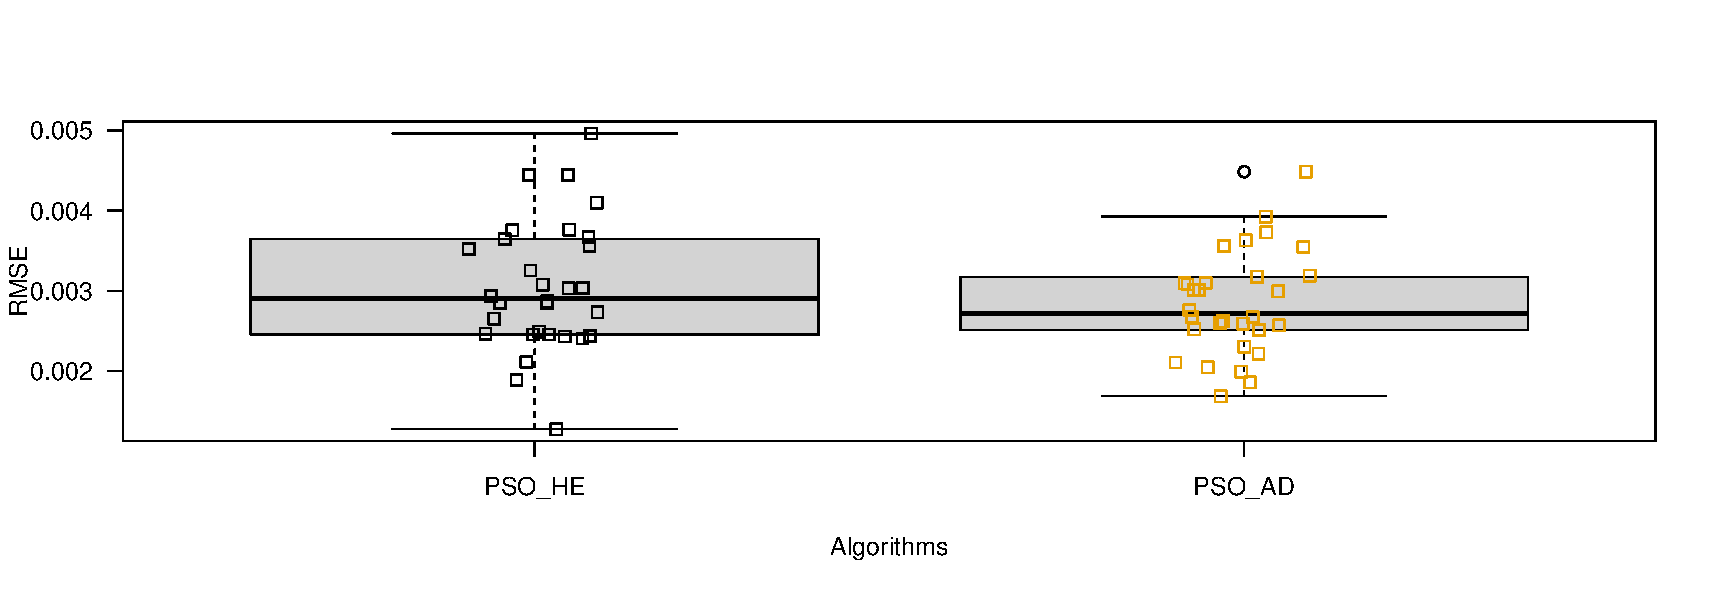
\includegraphics[angle=0,width=1\textwidth]{RplotAjusteParam.pdf}
  \caption{Box-plot of the data.}
  \label{fig:boxplot} 
\end{figure}

\section{Conclusions and Future Work}\label{sec:conclusions}

We presented a design and implementation of a distributed multi-swarm algorithm method to optimize the parameters of the MFs for a fuzzy controller.

We run experiments with two strategies, fuzzy adaptation and heterogeneous configurations of the algorithms.

We found that both strategies yield similar results.

As a next step, we could implement other parameter adaptation strategies.


%
% ---- Bibliography ----
%
% BibTeX users should specify bibliography style 'splncs04'.
% References will then be sorted and formatted in the correct style.
%
\bibliographystyle{splncs03_unsrt}
\bibliography{biblio}
%
%\begin{thebibliography}{8}

%\end{thebibliography}
\end{document}


***
****
We continue with our previous work, in which we optimized the parameters for a
fuzzy controller used for path tracking by an autonomous mobile robot. This
problem is particularly time-consuming because we could follow these three
steps to optimize this type of controller: First, we run one or more
simulations with the controller; this is time-consuming, then we measure the
controller's error in each simulation, calculate an average, and if we are not
satisfied with the results, we adjust the parameters and start again. That is
why designers of fuzzy controllers often use population-based metaheuristics to
adjust these parameters. However, even when using a metaheuristic, fuzzy
controller optimization continues to be time-consuming. We briefly explain the
multi-population multi-heuristic algorithm used in this paper. The authors more
extensively explain the algorithm in \cite{mancilla2022optimal}.

We propose an event-based, distributed algorithm that exchanges data between
processes using message queues for asynchronous communication (see Fig.
\ref{fig:Diagrams}). (1) We start the algorithm by executing a single task that
pushes a specified $n$ number of populations to the Population Queue. Each
population message contains the initial configuration and the type of
metaheuristic used by that particular population. The main idea is that each
process runs a metaheuristic for a small number of iterations on a population
received as a message and then pushes the resulting (evolved) population to the
Evolved Population Queue (4). (3) Workers take messages asynchronously to
process the data (populations). Each worker inside a container continuously
checks for messages in the Population Queue and, after receiving a population,
executes a metaheuristic on this population for several iterations. (4)
resulting populations from the Evolved Population Queue. (5-6) An essential
component of the architecture is the Combinator process, responsible for taking
the resulting populations from the Evolved Population Queue and, after reading
the message, stopping the algorithm if the number of function evaluations has
been reached or if a suitable solution was found.

However, the primary responsibility of this component is to migrate or combine
populations arriving from the Evolved Population Queue. The combination method
we propose in this work is as follows. We take the top two best solutions from
each population and insert them in a buffer that always keeps the top-k
solutions. Finally, we replace the two worst solutions for the population with
the buffer's current first and second-best solutions.

\begin{figure}
  \centering
  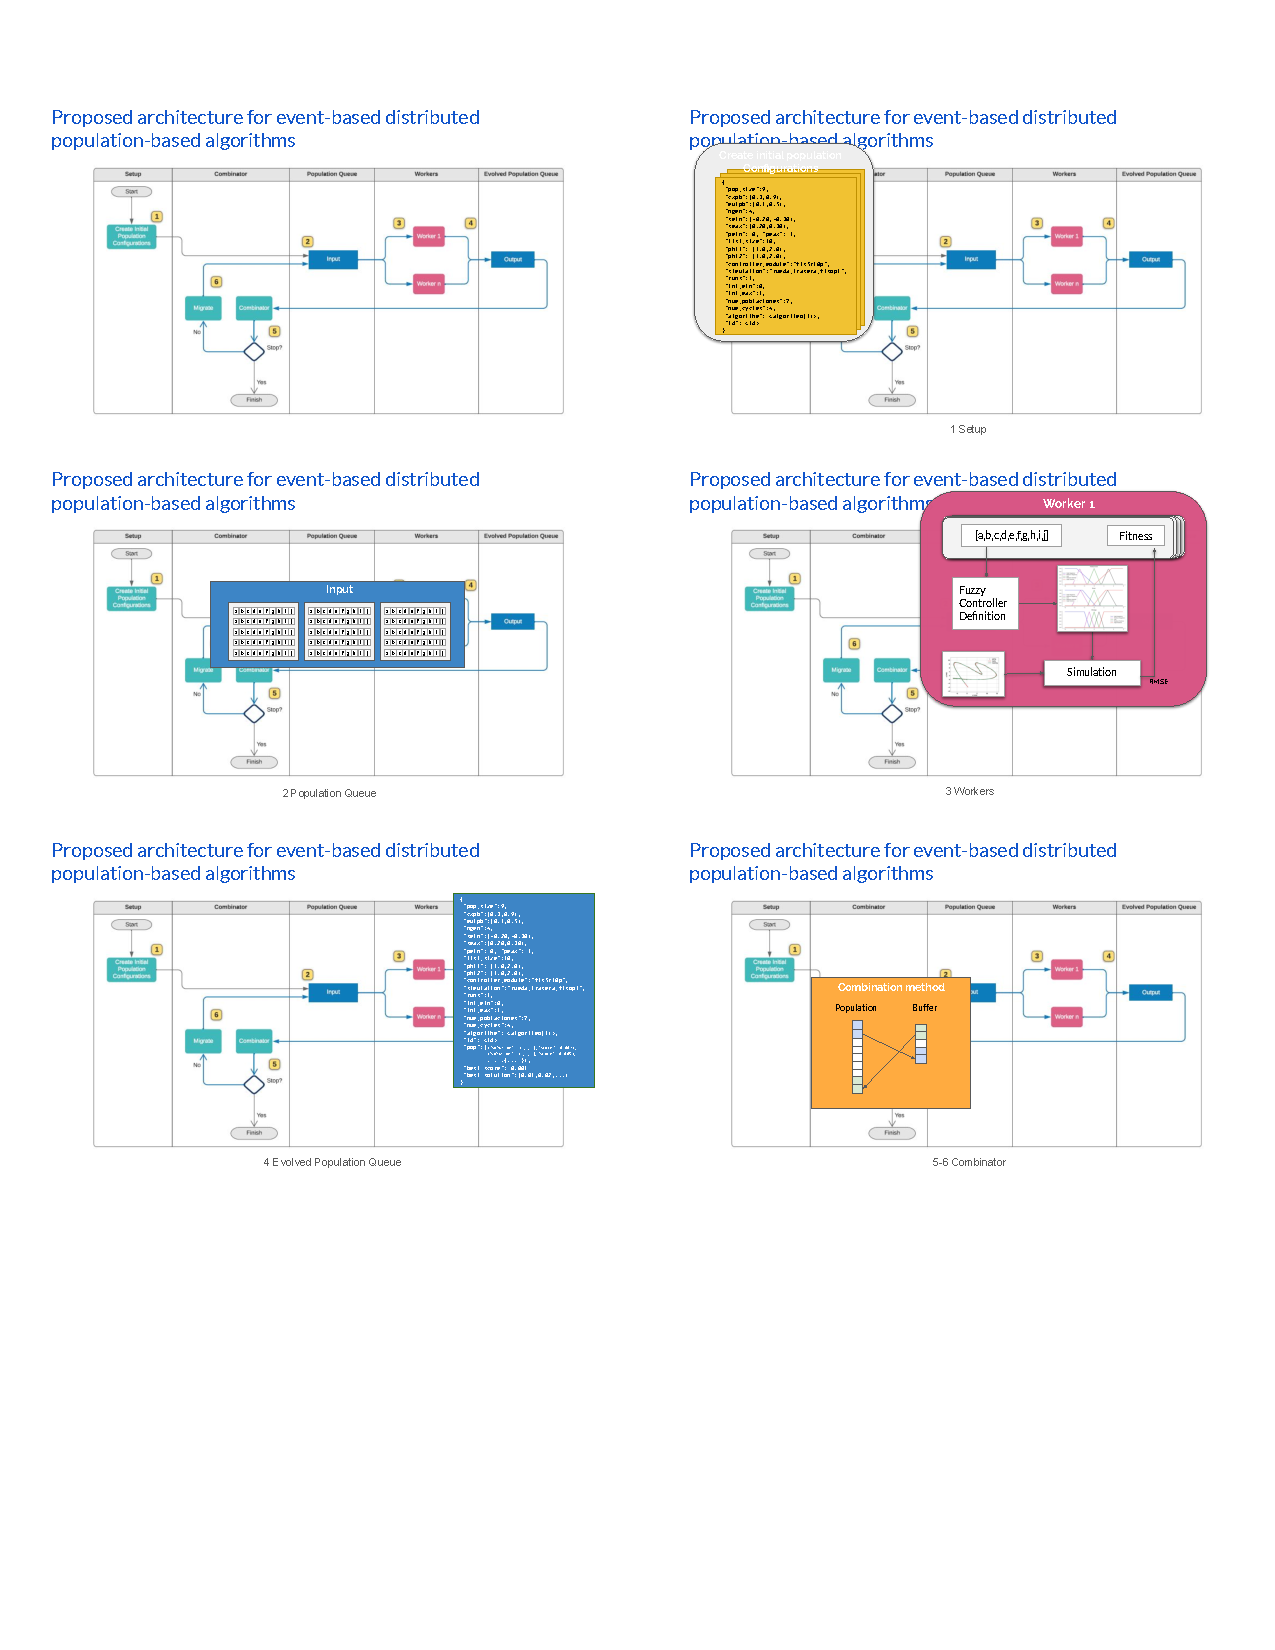
\includegraphics[angle=0,width=1\textwidth]{Diagrams}
  \caption{Proposed architecture for event-based distributed population-based algorithms.}
  \label{fig:Diagrams} 
\end{figure}

\begin{figure}[ht]
  \centering
  \begin{subfigure}{0.8\textwidth}
    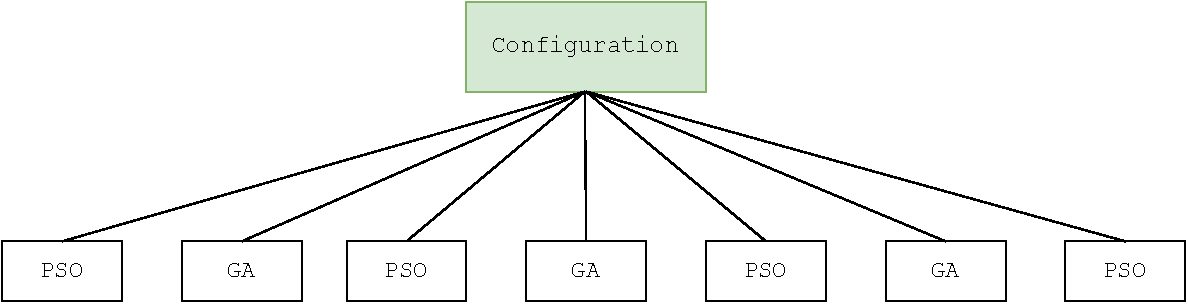
\includegraphics[angle=0,width=1\textwidth]{homogeneo}
    \caption{Homogeneous strategy.}
    \label{fig:s_homogeneo} 
  \end{subfigure}

  \begin{subfigure}{0.8\textwidth}
     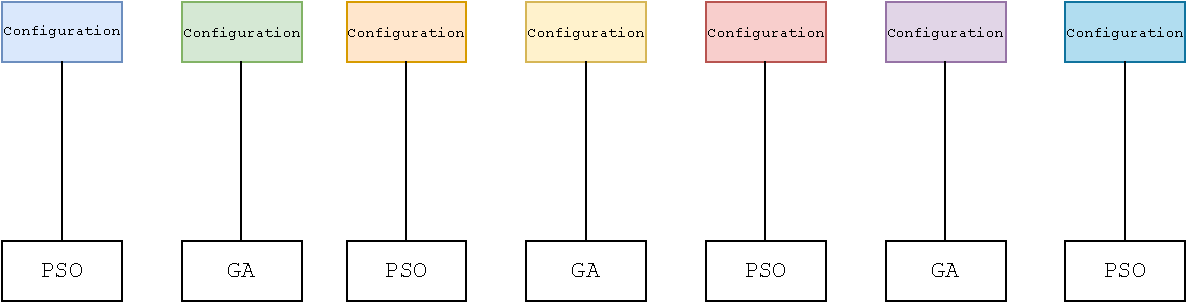
\includegraphics[angle=0,width=1\textwidth]{heterogeneo}
     \caption{Heterogeneous strategy.}
     \label{fig:s_heterogeneo} 
  \end{subfigure}
\caption{ Illustration of the type of strategies compared in this work.}
\label{fig:s_strategies}
\end{figure}

One of the problems of metaheuristics is establishing the initial values of the
algorithm's parameters. Usually, bio-inspired metaheuristics have parameters
that control how much the algorithm does an exploration or exploitation over
the search space \cite{yang2013swarm}. If the algorithm exploits too much, there is a higher risk of
premature convergence to a local minimum. On the other hand, if there is too
much exploration, the algorithm will search allmost randomly, constantly
changing the area of attention. A balance between the two types of search is
required to escape local minima while simultaneously doing a local search in a
promising area.

When we have several populations, we could use a strategy to
have some populations tending to exploration and others to exploitation. The
idea is that this strategy keeps a natural balance between the two extremes.
The problem remains: how do we set the parameters now that we have many more, a
set for each population? A simple heterogeneous strategy proposed by \cite{gong2011distributed} 
randomly sets each population's parameters. Although simple, the random
strategy has yielded promising results in other multi-population algorithms .
The other strategy found in the literature is using a single, well-balanced
configuration for each metaheuristic algorithm and repeating the same
configuration in all populations. In Fig. \ref{fig:s_strategies} on the top
image, we can see a representation of the homogenous strategy (Fig.
\ref{fig:s_homogeneo}) and the heterogeneous strategy at the bottom (Fig.
\ref{fig:s_heterogeneo}).

\subsection{Control Problem}\label{sub:fuzzy}

The benchmark control problem we use to validate our proposal is the rear-wheel
controller described by Paden \cite{paden_survey_2016}. In this control problem, we have as
input the error $e$ that is the distance between the rear wheel and the desired
trajectory. The error is positive if the wheel is to the left of the path and
negative if it is to the right. The second input is the angle between the
tangent at the nearest point in the trajectory and the bearing
vector $\theta_{e}$. The output is the angular velocity $\omega$. We take the
design of the controller from a previous work \cite{mancilla2022tracking} using five membership
functions for each input variable. We have two signs because the error and the
heading can be left or right. We are tuning the ten parameters defining each
MF. The fixed and variable parameters of the MFs are in Table \ref{tab:mfs}. We proposed a
controller with a total of twenty five fuzzy rules.

\begin{table}[htbp] \caption{ Parameters for the controller's MFs}
    \label{tab:mfs} \centering
    \begin{tabular}{cccc}
    \hline
     \textbf{Variable} & \textbf{Linguistic Value} & \textbf{MF}& \textbf{Parameters}  \\
    \hline
    $\theta_e$ & high negative  & $\mu_{trap}$  & $[-50, -5, -b, -b+c]$     \\ 
    $\theta_e$ & medium negative& $\mu_{tria}$  & $[-d-e, -d, -d+e]$     \\ 
    $\theta_e$ & low            & $\mu_{tria}$  & $[-a, 0, a]$     \\ 
    $\theta_e$ & medium positive& $\mu_{tria}$  & $[d-e, d, d+e]$     \\ 
    $\theta_e$ & high positive  & $\mu_{trap}$  & $[b-c, b, 5, 50]$ \\

    \hline
    $error$ & high negative  & $\mu_{trap}$  & $[-50, -5, -g, -g+h]$     \\ 
    $error$ & medium negative& $\mu_{tria}$  & $[-i-j, -i, -i+j]$     \\ 
    $error$ & low            & $\mu_{tria}$  & $[-f, 0, f]$     \\ 
    $error$ & medium positive& $\mu_{tria}$  & $[i-j, i, i+j]$     \\ 
    $error$ & high positive  & $\mu_{trap}$  & $[g-h, g, 5, 50]$ \\

    \hline
    $\omega$ & high negative  & $\mu_{trap}$  & $[-50, -5, -1, -0.5]$     \\ 
    $\omega$ & medium negative& $\mu_{tria}$  & $[-1, -0.5, 0]$     \\ 
    $\omega$ & low            & $\mu_{tria}$  & $[-0.5, 0, 0.5]$     \\ 
    $\omega$ & medium positive& $\mu_{tria}$  & $[0, 0.5,1]$     \\ 
    $\omega$ & high positive  & $\mu_{trap}$  & $[0.5, 1 ,5, 50]$     \\ 
    \hline
\end{tabular}
\end{table}

The fitness of each candidate solution, in this case, the fuzzy controller
generated with the parameterized MFs, is established by running three
simulations in these three paths (see Fig. \ref{fig:Routes}).

\begin{figure}
  \centering
  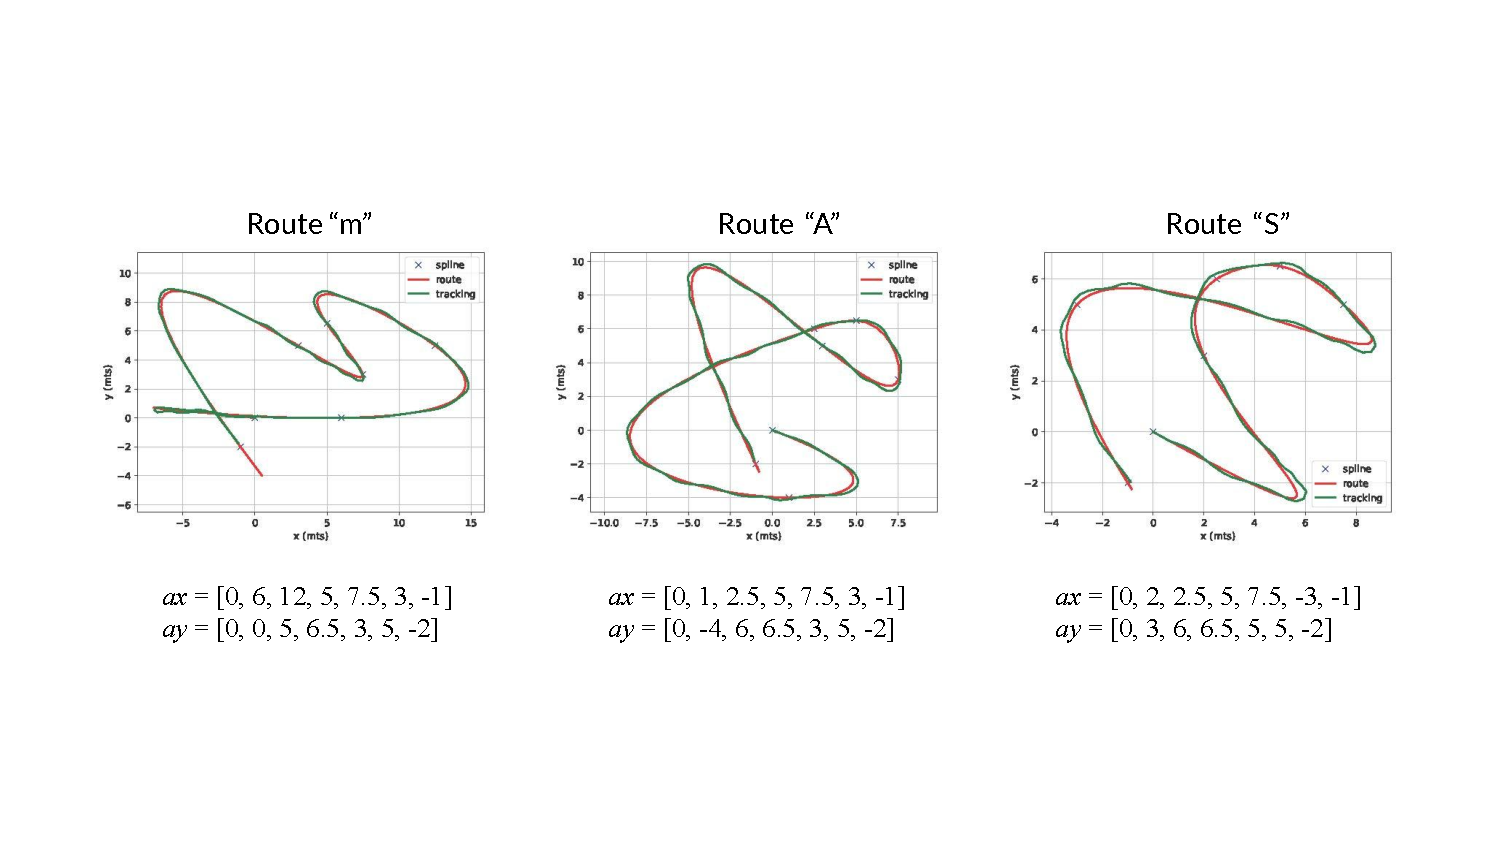
\includegraphics[angle=0,width=1\textwidth]{Routes}
  \caption{Paths used for fitness evaluation.}
  \label{fig:Routes} 
\end{figure}

\subsection{Setup}\label{sub:conf}

The distributed algorithms' parameters are shown in Table \ref{tab:alg_params}.
We configured the multi-population algorithm with seven populations of size
nine, this population size may seem small, but we need to remember that this is
a multi-population algorithm, so the total population size is estimated by
multiplying the population size by the number of sub-populations, in this case
the total size is 63. Each worker process will execute four iterations
(generations) of the algorithm, again the number of generations is small, but
this is by design. The small number of generations is required to distribute
the work among all worker processes. All populations will complete four cycles;
this means they will pass through the combinator module four times. We also
show the values we use to initialize the homogenous and heterogeneous
parameters.

Using interval notation, we defined a range from each parameter. We
can see that the interval includes the value specified for the homogenous
strategy in each parameter. For mutation probability in GAs, we set the value
at 0.3, and the range for random values is between 0.1 and 0.5. We experimented
with widening the range but did not receive better results. We repeated the
same setup for the other parameters. We wanted to maintain the speed limit sign
for PSO, so we established a range of $[-0.20, -0.30]$ and $[0.20, 0.30]$,
respectively. 

\begin{table}[htbp] 
\small
\caption{Parameter values for the algorithms compared}\label{tab:alg_params}
\begin{tabular}{l l l l}
\hline
\textbf{Algorithm} & \textbf{Parameter}	& \textbf{Fixed Value} & \textbf{Random Range}\\ 
                   &                    &                      &      [min,max]\\ \hline
GA & Selection & Tournament Selection (k =3)  \\
& Mutation  & Gaussian ($\mu=0.0$ and $\sigma=0.2$)  \\
& Mutation probability  &  0.3 &  [0.1, 0.5] \\
& Crossover  & One point (probability = 0.7) &  [0.3, 0.9]   \\
\hline
PSO & Topology & Fully connected  \\
& Speed limit & Min=-0.25 & Min=[-0.20, -0.30] \\
&             & Max=0.25 &  Max=[0.20, 0.30]  \\
& Cognitive and Social & $C_1=2,C_2=2$ &  [1.0, 2.0]  \\
\hline
Polutations& Pop Size &  9  \\
& Populations & 7 \\
& Iterations & 4 \\
& Cycles & 4   \\
& \#Func. Eval. & 1008 \\
\hline
\end{tabular}
\end{table}

\section{Results}\label{sec:results}

In Table \ref{tab:rmse}, we show the results of the experiments. Results with
parameters with random values are compared with the distributed
versions with fixed parameters found in our previous work.

We note that the distributed PSO with random parameters implementation
yields better results than the distributed homogeneous parameters on average.
Here we show the average error obtained in 30 runs. Here we show the best RMSE
obtained by the best fuzzy controller found in each run.

\begin{table}[ht]
    \caption{Results the best RMSE.} 
    \label{tab:rmse}
    \centering
    \setlength{\tabcolsep}{3pt}
    \begin{tabular}{|c|c|c|c|c|c|c|}
      \hline
      \multicolumn{7}{|c|}{RMSE} \\ \hline
      & \multicolumn{3}{|c|}{Homogeneous Parameters}  & \multicolumn{3}{c|}{ Heterogeneous Parameters} \\
         \cline{2-7}

             & GA         & PSO        & PSO-GA       & GA        & PSO        & PSO-GA  \\ \hline
    AVERAGE   & 0.01091   & 0.00645    & 0.00656      & 0.01029    & 0.00632     & 0.00634\\ \hline
    STDDEV    & 0.00600   & 0.00148	   & 0.00185      & 0.00332    & 0.00165     & 0.00135\\ \hline   
    MEDIAN    & 0.00955	 	& 0.00643	   & 0.00625      & 0.01021    & 0.00628     & 0.00610\\ \hline 
    MIN       & 0.00384	  & 0.00360	   & 0.00336      & 0.00399    & 0.00310     & 0.00388\\ \hline   
    MAX       & 0.03455	  & 0.01000    & 0.01168      & 0.01584    & 0.00891     & 0.00889\\ \hline    
      \end{tabular}
\end{table}

In Table \ref{tab:time} we show the time needed to complete each run in
seconds. When comparing the time required to complete each execution of the
algorithms, there is no substantial difference between versions. As expected,
the distributed version with random parameters turned out similar to that with
fixed parameters. An interesting case is the GA that took less time to complete
in the heterogeneous strategy. This shortening in time could be related to the
time it takes for a simulation to complete. Because we terminate the simulation
early if the robot loses track of the trajectory, the time required to complete
the simulations for a population of incapable individuals could take less time.
This result, however, does not happen in the PSO case, where the times are
similar. 

\setlength{\tabcolsep}{3pt}
\begin{table}[ht]
  \caption{Results the time in seconds needed to complete each run.}
  \label{tab:time}
  \centering
  \begin{tabular}{|c|c|c|c|c|c|c|} 
    \hline
    \multicolumn{7}{|c|}{Time (Sec.)} \\ \hline
        & \multicolumn{3}{|c|} {Homogeneous Parameters} &  \multicolumn{3}{c|}{Heterogeneous Parameters} \\ 
        \cline{2-7}  
             & GA         & PSO        & PSO-GA       & GA        & PSO        & PSO-GA  \\ \hline
  AVERAGE    & 421.6722   & 415.6491   & 431.5258     & 395.7506  & 415.7994   & 409.9042     \\ \hline
  STDDEV     &  28.5406   &  23.4744   &  22.6012     &  26.5488  &  20.4787   &  24.8533     \\ \hline   
  MEDIAN     & 417.8451   & 412.6850   & 432.3661     & 392.8096  & 414.6650   & 408.4821     \\ \hline 
  MIN        & 364.6546   & 365.8164   & 394.6160     & 340.6548  & 374.8318   & 372.2037     \\ \hline   
  MAX        & 526.7686   & 467.4715   & 478.8072     & 461.4638  & 461.9615   & 465.2711     \\ \hline    
   \end{tabular}
 \end{table}

We did the statistical Ztest, comparing the same algorithms but with
homogeneous parameters that are those of the column that we see on the left
side and the algorithms with heterogeneous parameters that we see in the upper
row. We concluded that there is not enough evidence to reject the null
hypothesis. The p-value results show that it is not within the acceptable
confidence interval. We show in Table \ref{tab:ztest}.

 \begin{table}[ht]
  \caption{Statistical Ztest.}
  \label{tab:ztest}
  \centering
  \setlength{\tabcolsep}{8pt}
  \begin{tabular}{|c|c|c|c|c|}
    \hline
    \multicolumn{5}{|c|}{  p-values,  Z-test $\alpha$=0.05,  independent samples,  unequal variances,  30 samples  }  \\ [1ex] \hline
    \multicolumn{2}{|c|}{} & \multicolumn{3}{c|} {Heterogeneous Parameters} \\ \hline
             &                                      &  GA            &  PSO         & PSO-GA  \\ 
             &  $H_a$ : $\mu_{eAi}$ $>$ $\mu_{eAj}$ &  X:0.01029    & X:0.00632     & X:0.00634 \\ 
             &                                      & SD:0.00332    & SD:0.00165    & SD:0.00135 \\  
             \hline
  \multirow{9}{*}{\begin {sideways}Homogeneous Params \end{sideways}} 
                      & GA     & \cellcolor{lightgray}        &  & \\ 
             &  X : 0.01091   & 0.3119 \cellcolor{lightgray} &  & \\ 
             & SD : 0.00600   & \cellcolor{lightgray}        &  & \\ 
             \cline{2-5}
                     & PSO     &        & \cellcolor{lightgray}        & \\ 
             &  X : 0.00645   &        & 0.3819 \cellcolor{lightgray} & \\
             & SD : 0.00148   &        & \cellcolor{lightgray}        & \\ 
             \cline{2-5}  
                    & PSO-GA   &        &       & \cellcolor{lightgray}        \\ 
             &  X : 0.00656   &        &       & 0.3085 \cellcolor{lightgray} \\ 
             & SD : 0.00185   &        &       & \cellcolor{lightgray}        \\
              \hline    
  \end{tabular}
\end{table}

We show a box-plot of the data in Fig.\ref{fig:boxplot}, and we can see that
there is no significant difference between the median of the same algorithms.

\begin{figure}[ht]
  \centering
  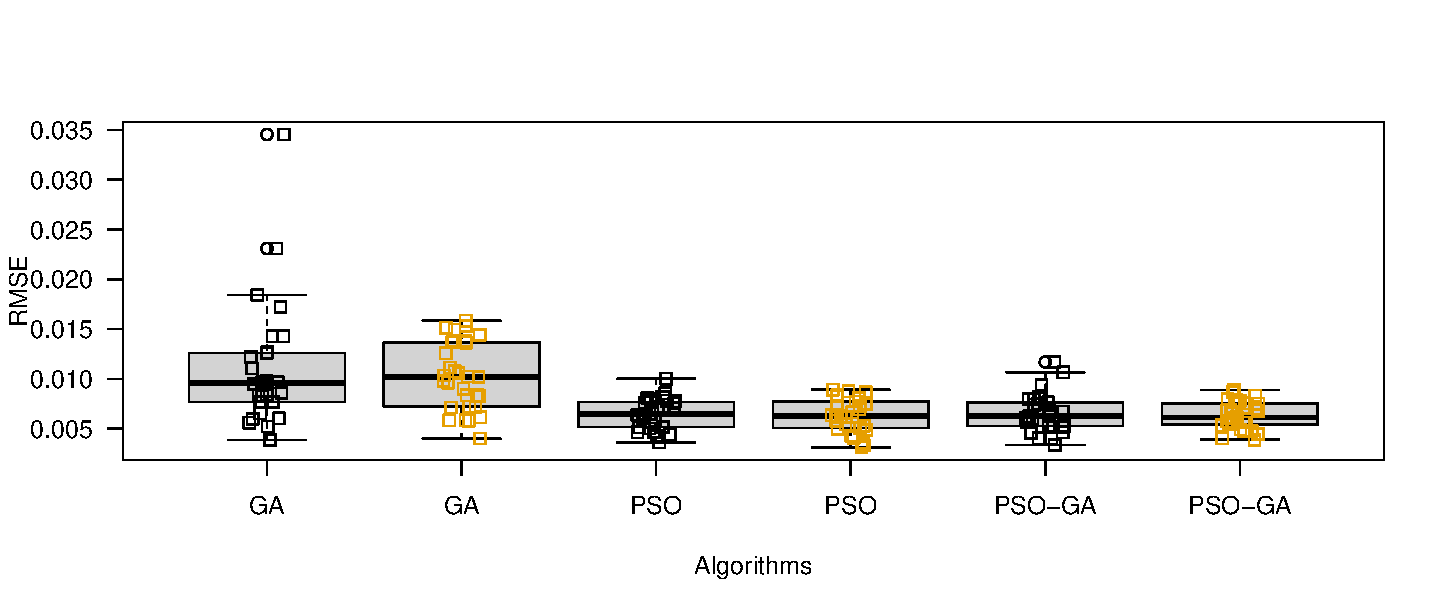
\includegraphics[angle=0,width=1\textwidth]{boxplot}
  \caption{Box-plot of the data.}
  \label{fig:boxplot} 
\end{figure}

\section{Conclusions and Future Work}\label{sec:conclusions}

In conclusion we presented a design and implementation of a distributed 
multi-population, multi-algorithm method to optimize the parameters of 
the MFs for a fuzzy controller.

We run experiments with both heterogeneous and homogeneous configurations
of the algorithms.

Preliminary results show that a distributed execution with homogeneous 
parameters gives similar results to a distributed implementation with 
random parameters in a similar time.  By using random heterogeneous 
parameters, we do not spend the time needed to find a suitable set of
parameters, we only need to specify a range.

For future work, we need to run the experiments in a computer with 
more cores or on the cloud. As a next step,  we could implement 
other optimization algorithms. Also, there are other parameters that 
are important like the poplulation size and the number of iterations.
Moreover, we can also investigate if a dynamic tuning of parameters yields 
better results. For instance, the Combinator process could adjust the parameters 
in each iterations taking into account certain metrics of the population like 
the diversity or the average fitness.

%
% ---- Bibliography ----
%
% BibTeX users should specify bibliography style 'splncs04'.
% References will then be sorted and formatted in the correct style.
%
\bibliographystyle{splncs03_unsrt}
\bibliography{biblio}
%
%\begin{thebibliography}{8}

%\end{thebibliography}
\end{document}
